\documentclass[paper=a4, fontsize=11pt]{scrartcl}
\usepackage[T1]{fontenc}
\usepackage{fourier}

\usepackage[english]{babel}															% English language/hyphenation
\usepackage[protrusion=true,expansion=true]{microtype}	
\usepackage{amsmath,amsfonts,amsthm} % Math packages
\usepackage[pdftex]{graphicx}	
\usepackage{url}
\usepackage{hyperref}


%%% Custom sectioning
\usepackage{sectsty}
\allsectionsfont{\centering \normalfont\scshape}
\usepackage{subfigure}
\usepackage{comment}


%%% Custom headers/footers (fancyhdr package)
\usepackage{fancyhdr}
\pagestyle{fancyplain}
\fancyhead{}											% No page header
\fancyfoot[L]{}											% Empty 
\fancyfoot[C]{}											% Empty
\fancyfoot[R]{\thepage}									% Pagenumbering
\renewcommand{\headrulewidth}{0pt}			% Remove header underlines
\renewcommand{\footrulewidth}{0pt}				% Remove footer underlines
\setlength{\headheight}{13.6pt}


%%% Equation and float numbering
%\numberwithin{equation}{section}		% Equationnumbering: section.eq#
%\numberwithin{figure}{section}			% Figurenumbering: section.fig#
%\numberwithin{table}{section}				% Tablenumbering: section.tab#


%%% Maketitle metadata
\newcommand{\horrule}[1]{\rule{\linewidth}{#1}} 	% Horizontal rule

\title{
		%\vspace{-1in} 	
		\usefont{OT1}{bch}{b}{n}
		\normalfont \normalsize \textsc{CS650 - Computer Vision} \\ [25pt]
		\horrule{0.5pt} \\[0.4cm]
		\huge Programming Lab 4 \\ Pattern Recognition Basics \\
		\horrule{2pt} \\[0.5cm]
}
\author{
		\normalfont 								\normalsize
        Daqing Yi\\[-3pt]		\normalsize
        \today
}
\date{}


%%% Begin document
\begin{document}
\maketitle

\begin{comment}
prepare a brief writeup to submit.
Your writeup should document your features and your algorithms as well as describe any observations you have made and ideas you have for how to improve the results.
Don't forget to document your code.

Descriptor
compactness, rectangularity, eccentricity, moments, elongation, psi-s curves, profiles, holes, corners, etc.
\end{comment}

\section{Introduction}
\label{sec:intro}

This lab implements a basic pattern recognition on the objects in binary images.
The implementations are written in Python.
CV2 (open CV) is used for reading image files into data arrays.
Numpy is used for array operations.
Matplotlib is used for visualizing data.

In this lab, the objects are firstly extracted from the image.
The features of the object are quantized into points in feature space.
A minimum distance classifier is used to separate the objects into five classes by shape features.
The results are also tested on other image files to verify generalization capability.

\section{Object isolation}
\label{sec:object_isolation}

The test image files are firstly loaded into binary image.
The binary image is maintained by a \textbf{PixelGraph} class in \emph{PixelGraph.py}.
Connected-Component labeling \footnote{\url{http://en.wikipedia.org/wiki/Connected-component_labeling}}
is used to isolate the objects from binary image.
Each 
The implementation follows the ``two-pass algorithm'' described in \cite{wiki:connected_component_labeling}.
A \textbf{ConnectedComponentMgr} in \emph{ConnectedComponent.py} is used to maintain the connected components found.
Each component is assigned an index as ID by sequence.
Seome examples are given in Figure \ref{fig:obj_iso}.

\begin{figure}[h]
\centering
\subfigure[Object Index 2 of \emph{shapes.pgm}]{
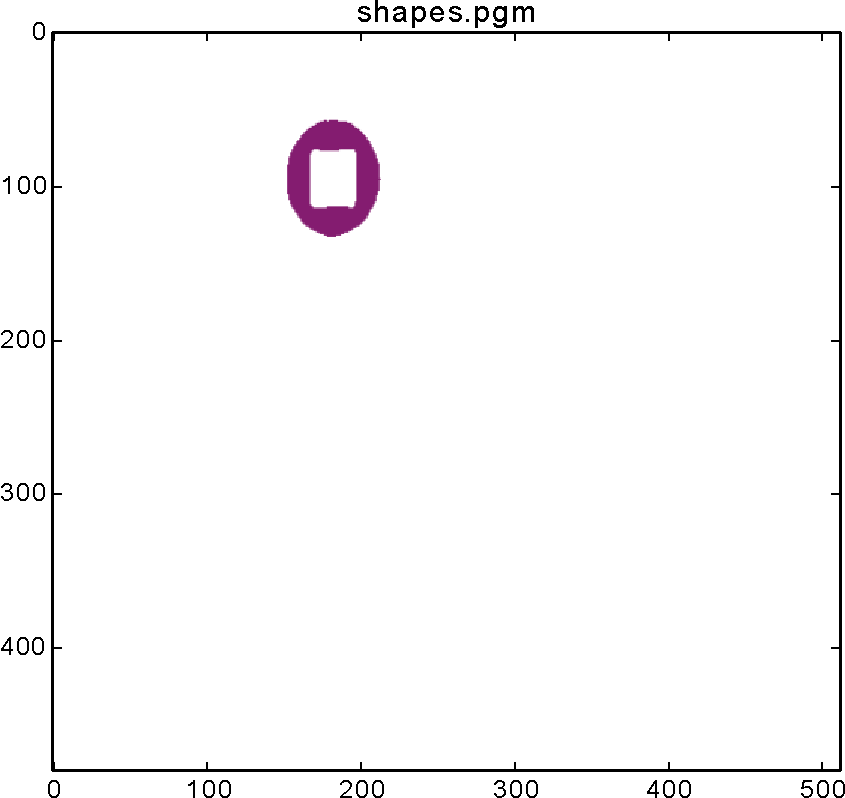
\includegraphics[width=.3\textwidth]{./figure/shapes_obj2} 
\label{fig:obj_iso:01} } 
\subfigure[Object Index 3 of \emph{train1.pgm}]{
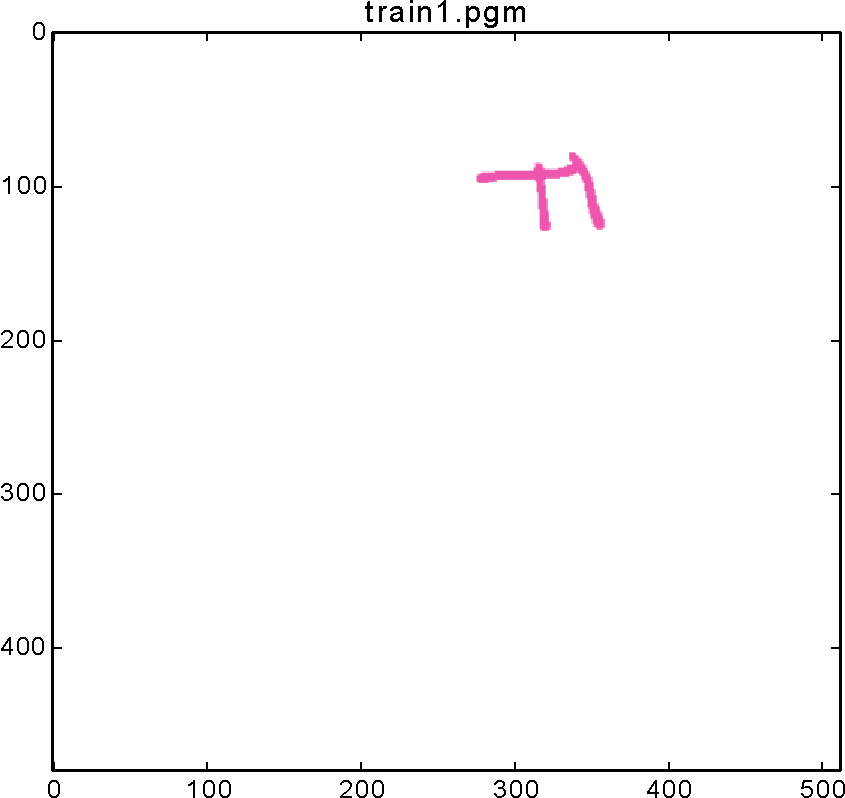
\includegraphics[width=.3\textwidth]{./figure/train1_obj3} 
\label{fig:obj_iso:02} } 
\subfigure[Object Index 4 of \emph{match1.pgm}]{
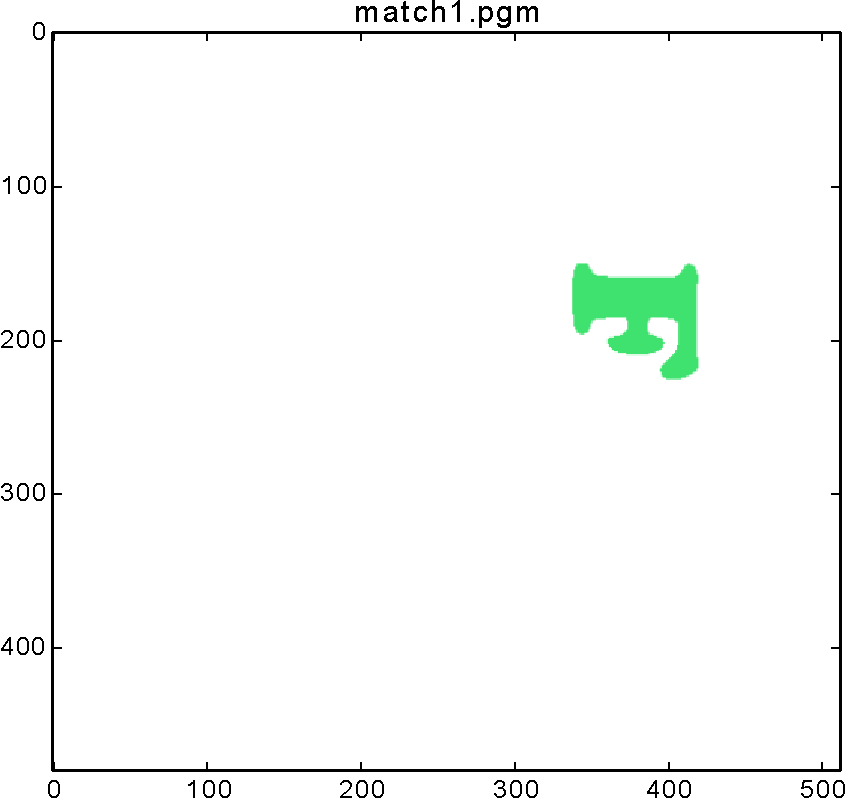
\includegraphics[width=.3\textwidth]{./figure/match1_obj4} 
\label{fig:obj_iso:03} } 
\caption{Object isolation.}
\label{fig:obj_iso}
\end{figure}

\begin{figure}[h]
\centering
\subfigure[Object Index 2 of \emph{shapes.pgm}]{
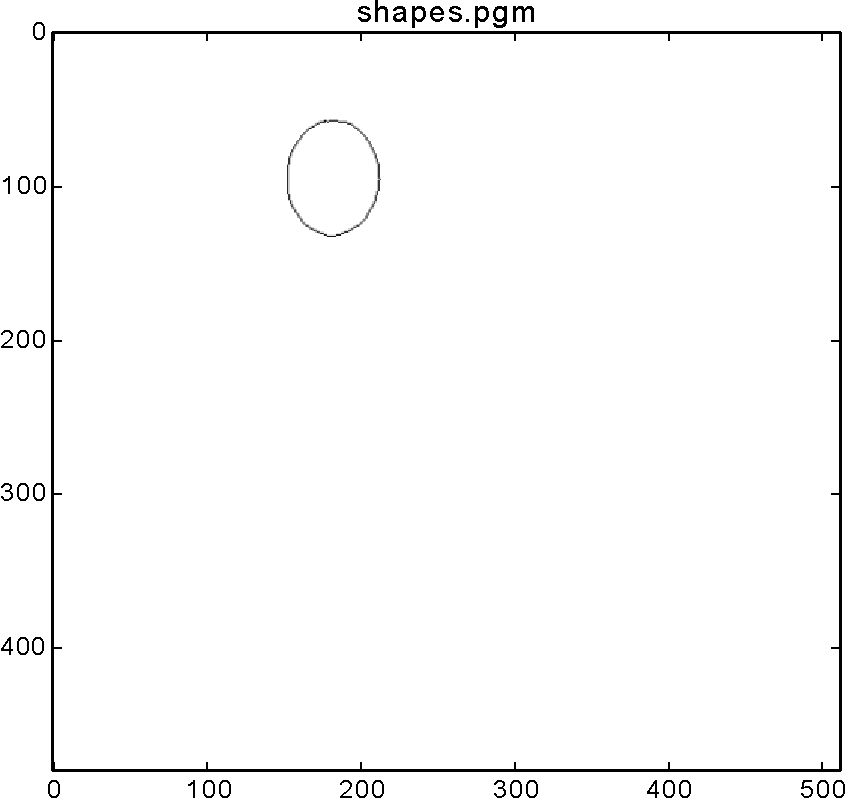
\includegraphics[width=.3\textwidth]{./figure/shapes_cc2} 
\label{fig:obj_cc:01} } 
\subfigure[Object Index 3 of \emph{train1.pgm}]{
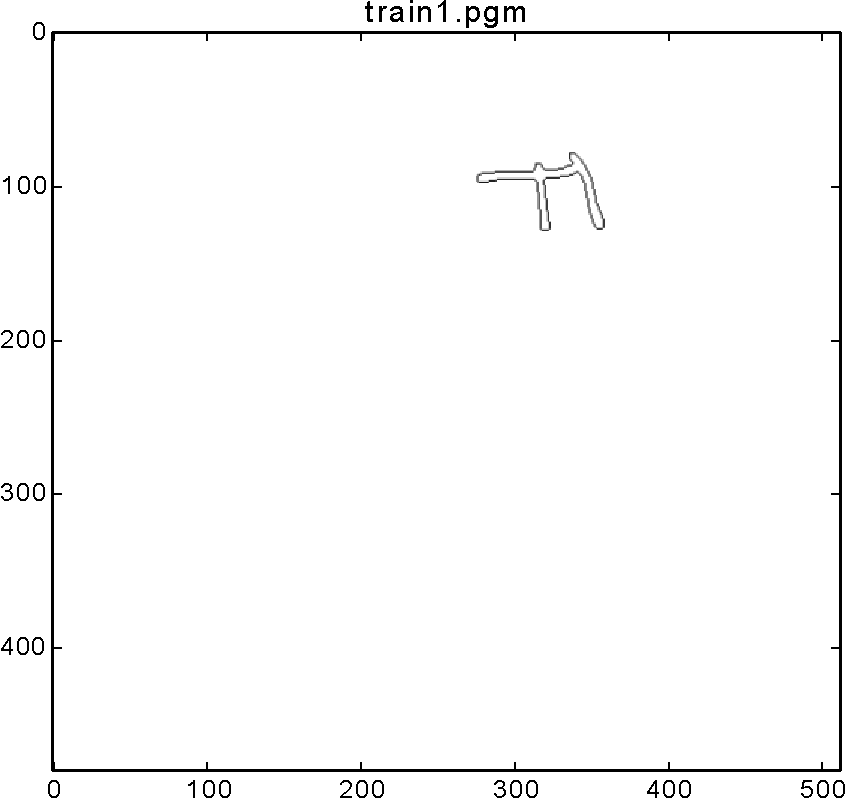
\includegraphics[width=.3\textwidth]{./figure/train1_cc3} 
\label{fig:obj_cc:02} } 
\subfigure[Object Index 4 of \emph{match1.pgm}]{
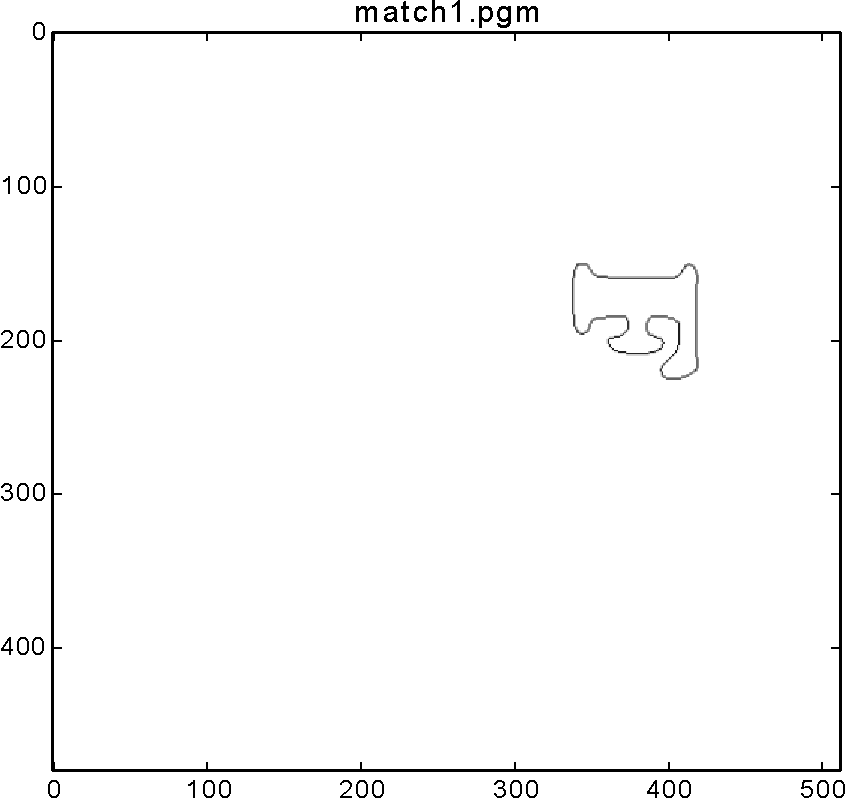
\includegraphics[width=.3\textwidth]{./figure/match1_cc4} 
\label{fig:obj_cc:03} } 
\caption{Contour finding.}
\label{fig:obj_cc}
\end{figure}

\section{Feature extraction}
\label{sec:feature_extraction}

A \emph{ShapeDescriptor} class in \emph{ShapeDescriptor.py} is used to generate shape features of a connected component.
In this label, the extracted features are listed as following.

\begin{itemize}
\item \textbf{Compactness} 

Compactness indicates how compact a shape is, which is measured by $ \mbox{perimeter}^{2} / \mbox{area} $.
$ \mbox{area} $ is counted by the pixel number.
$ \mbox{perimeter} $ is calculated from the contour. 
The contour is in the form of the chain code \footnote{\url{http://en.wikipedia.org/wiki/Chain_code}}. 
The algorithm is implemented following \cite{chaincode}.
The contours found can be used to calculate the perimeter of the object.
Figure \ref{fig:obj_cc} shows how the contours of the objects are like.,

\item \textbf{Rectangularity} 

Rectanglarity indicates how close a shape to a rectangle.
It is defined by the ration of the area of the object and the area of its minimum bounding rectangle.

\begin{figure}[h]
\centering
\subfigure[Convex hull]{
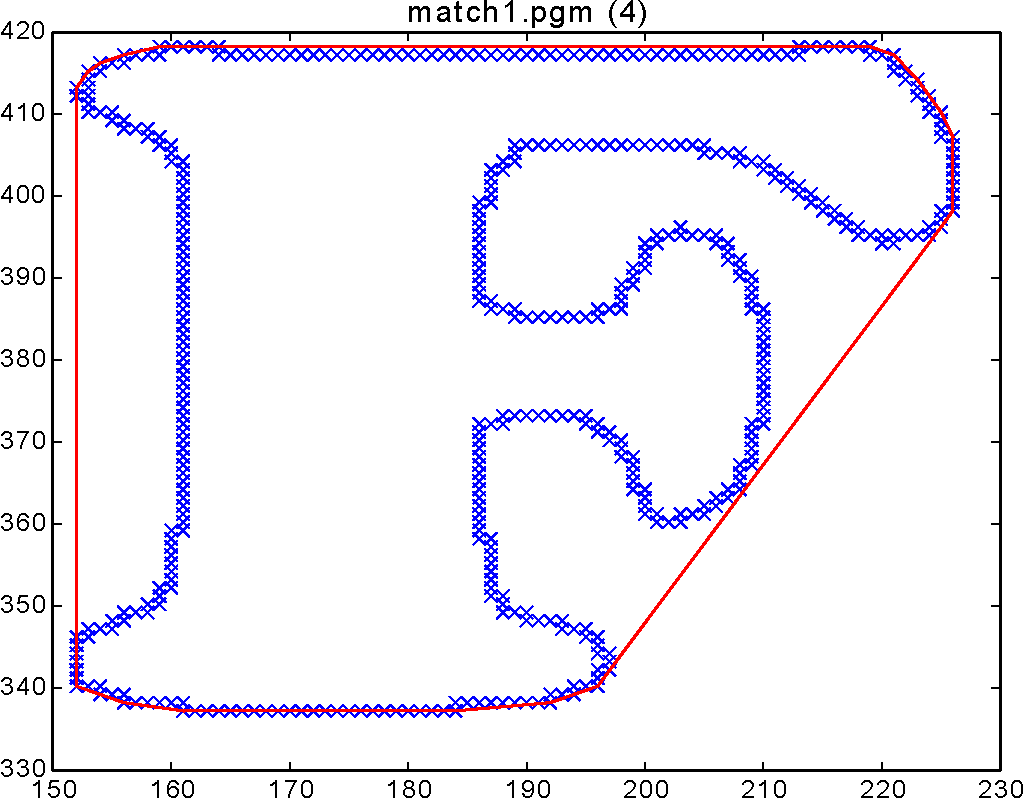
\includegraphics[width=.3\textwidth]{./figure/match1_convex_hull_4} 
\label{fig:convex_hull} } 
\subfigure[Minimum bounding rectangle]{
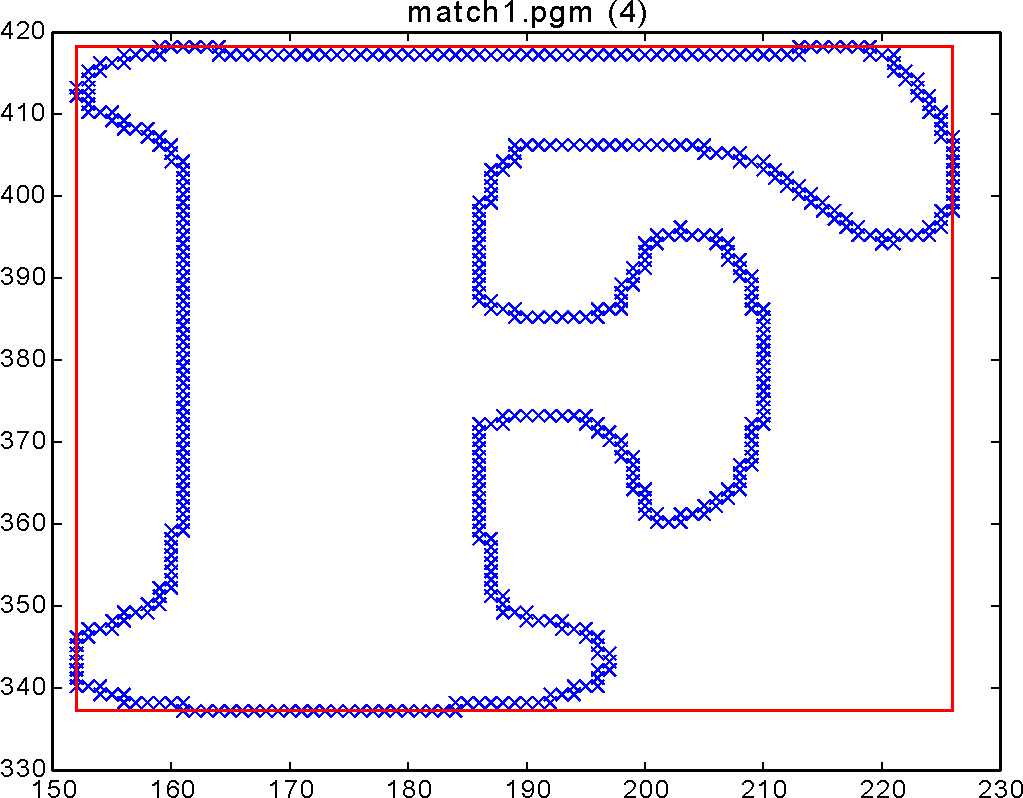
\includegraphics[width=.3\textwidth]{./figure/match1_min_rect_4} 
\label{fig:min_bound_box} } 
\caption{Convex hull and minimum bounding rectangle.}
\label{fig:convex_hull_min_bound_box}
\end{figure}

\item \textbf{Eccentricity}



\item \textbf{Elongation}

\item \textbf{Aspect ratio}

\item \textbf{Hole area ratio}

\item \textbf{Moments}

\item \textbf{Psi-s curves}
\item \textbf{Profiles}
\item \textbf{Holes}
\item \textbf{Corners}
\end{itemize}

\section{Minimum distance classifier}
\label{sec:classifier}

A minimum distance classifier is used to classify the objects by features.
Because a 5 separate pattern clustering is required.
K-means clustering is firstly used to find the mean of each cluster.
The means are then used by a minimum-distance classifier.
In this multiple classes case, there is a single linear discriminant $ g_{i} ( \mathbf{x} ) $ for each class $ \omega_{i} $.
The class $ \omega_{i} $ is assigned to $ \mathbf{x} $ if $ \forall j \neq i, g_{i} ( \mathbf{x} ) > g_{j} ( \mathbf{x} ) $.
$ g_{i}( \mathbf{x} ) $ is defined as 
\begin{equation}
g_{i}( \mathbf{x} ) = \mathbf{x}^{T} \mathbf{m}_{i} - \frac{1}{2} \mathbf{m}_{i}^{T} \mathbf{m}_{i}.
\end{equation}
Because minimizing $ || \mathbf{x} - \mathbf{m}_{i} || $ is equivalent to maximizing $ \mathbf{x}^{T} \mathbf{m}_{i} - \frac{1}{2} \mathbf{m}_{i}^{T} \mathbf{m}_{i} $.
Figure \ref{fig:min_dist_classifer} gives an example of the minimum distance classifier that is applied on randomly generated 2D data.

\begin{figure}
\centering
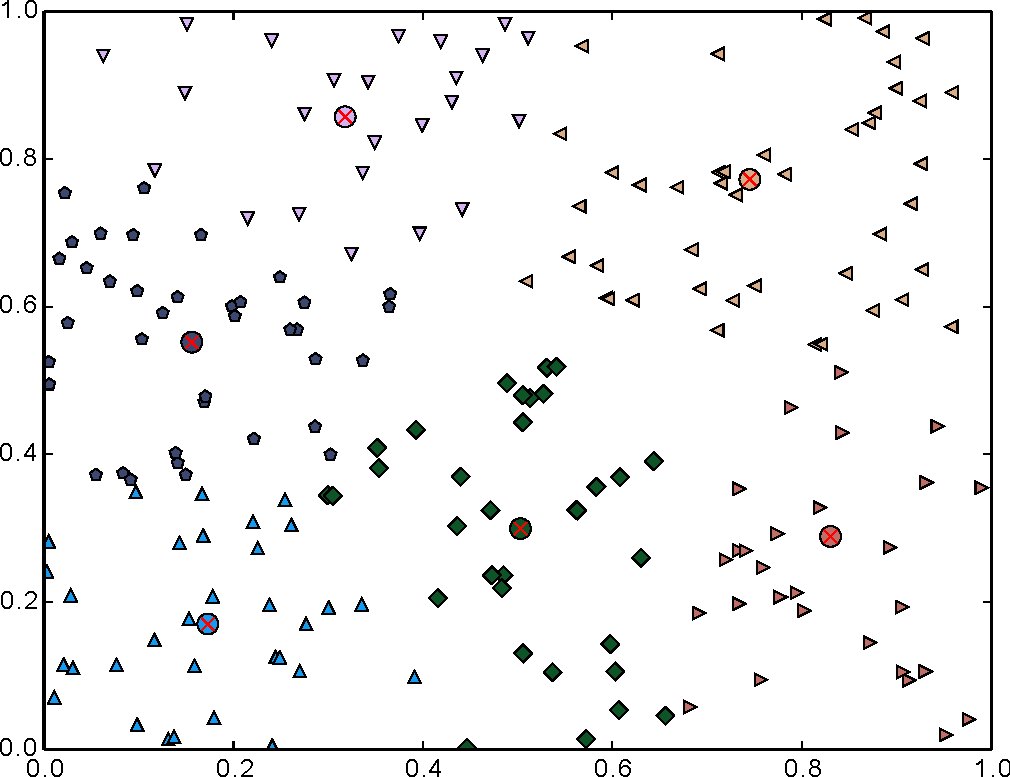
\includegraphics[width=0.7\linewidth]{./figure/kmean}
\caption{Minimum Distance classifier.}
\label{fig:min_dist_classifer}
\end{figure}

\section{Pattern recognition}
\label{sec:pattern_recognition}


\begin{figure}[h]
\centering
\subfigure[Training]{
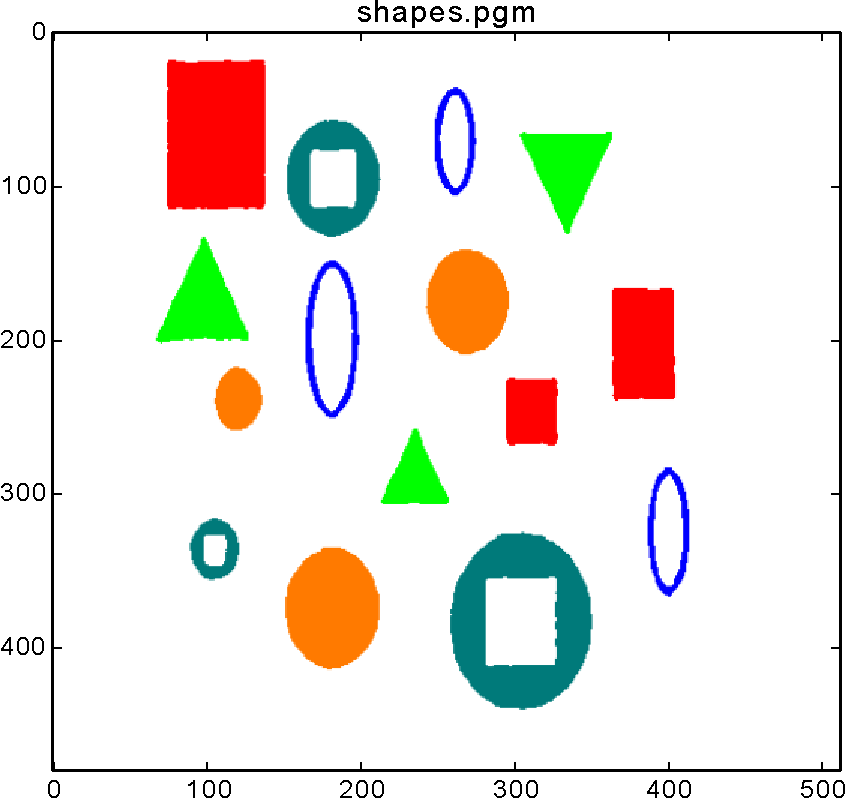
\includegraphics[width=.45\textwidth]{./figure/shapes_pgm-0} 
\label{fig:class:01:train} } 
\subfigure[Testing]{
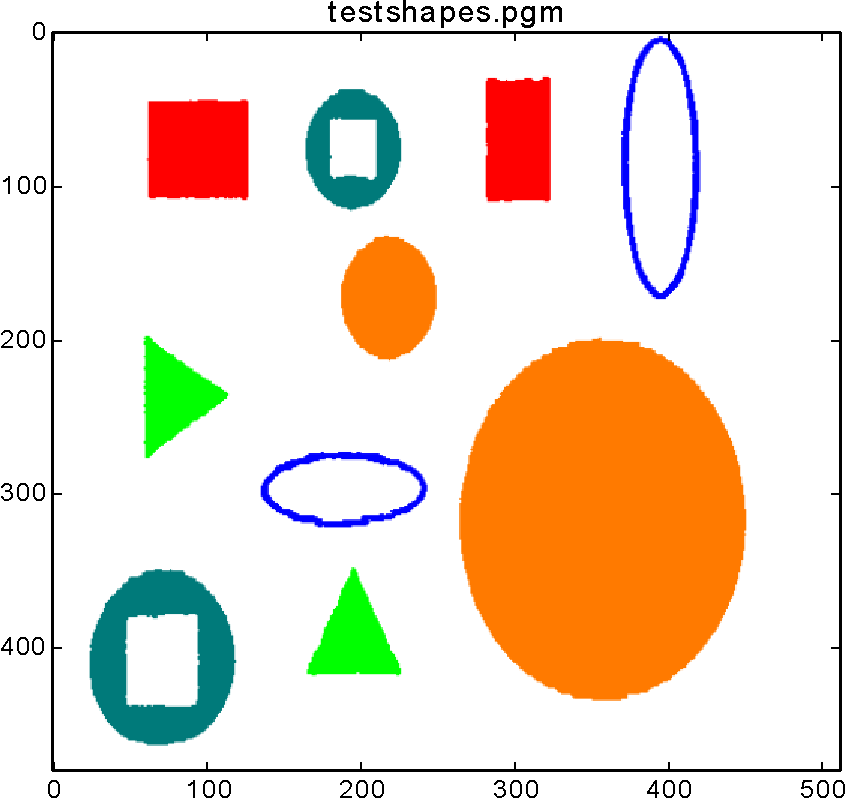
\includegraphics[width=.45\textwidth]{./figure/testshapes_pgm-0} 
\label{fig:class:01:test} } 
\caption{Classifications on \emph{shapes.pgm} and \emph{testshapes.pgm}.}
\label{fig:class:01}
\end{figure}

\begin{figure}[h]
\centering
\subfigure[Training 1]{
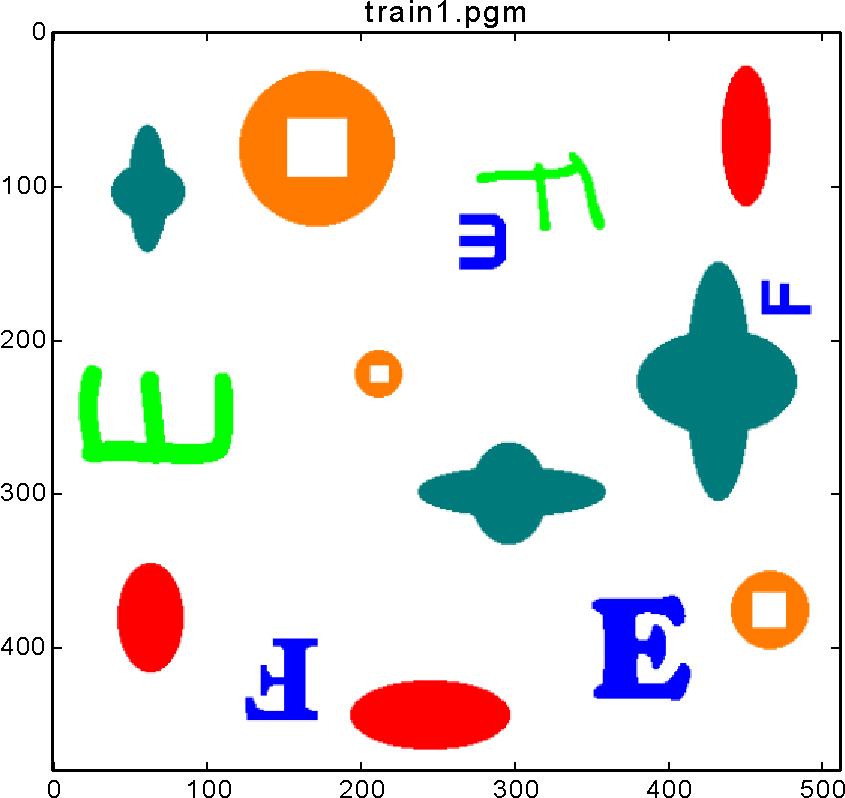
\includegraphics[width=.45\textwidth]{./figure/train1_pgm-0} 
\label{fig:class:02:train1} } 
\subfigure[Training 2]{
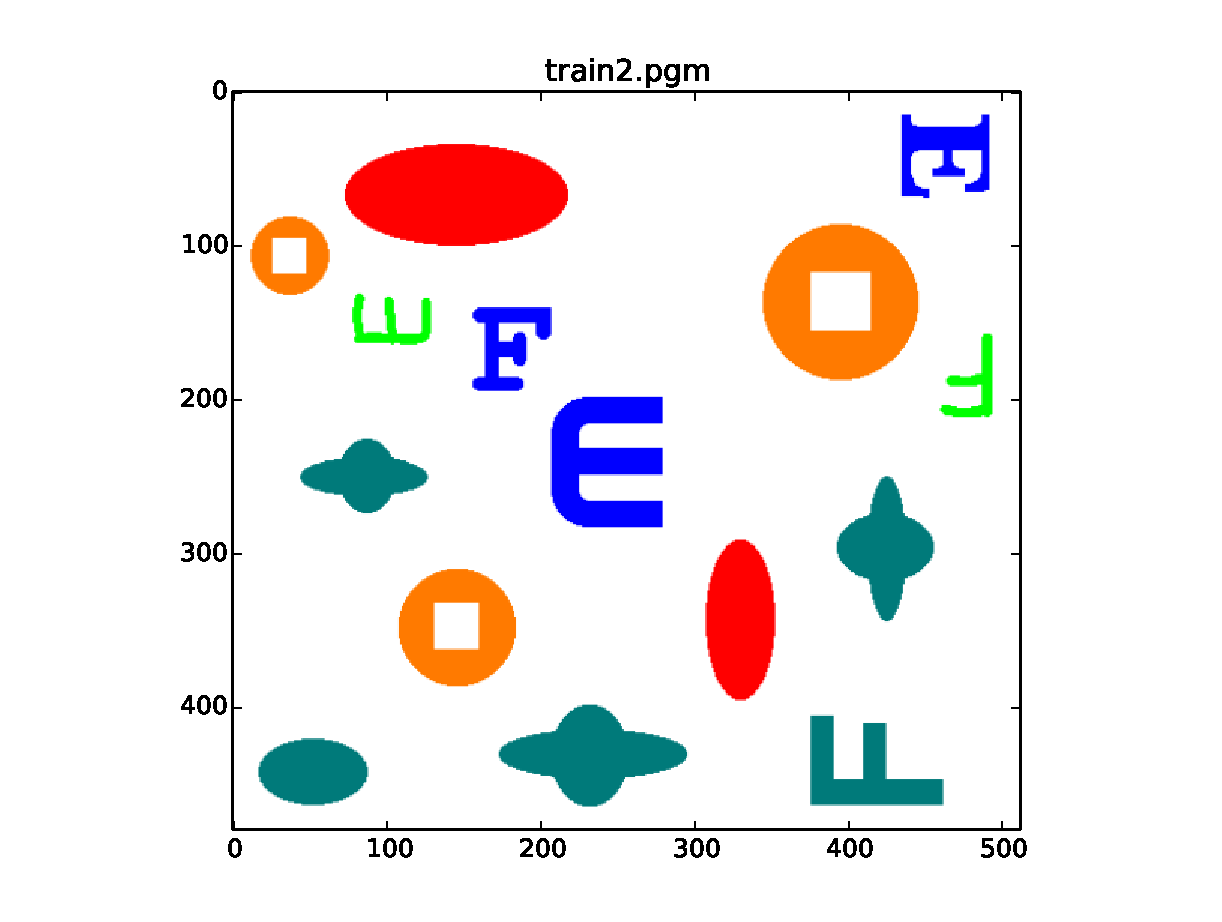
\includegraphics[width=.45\textwidth]{./figure/train2_pgm-0} 
\label{fig:class:02:train2} }
\\
\subfigure[Testing 1]{
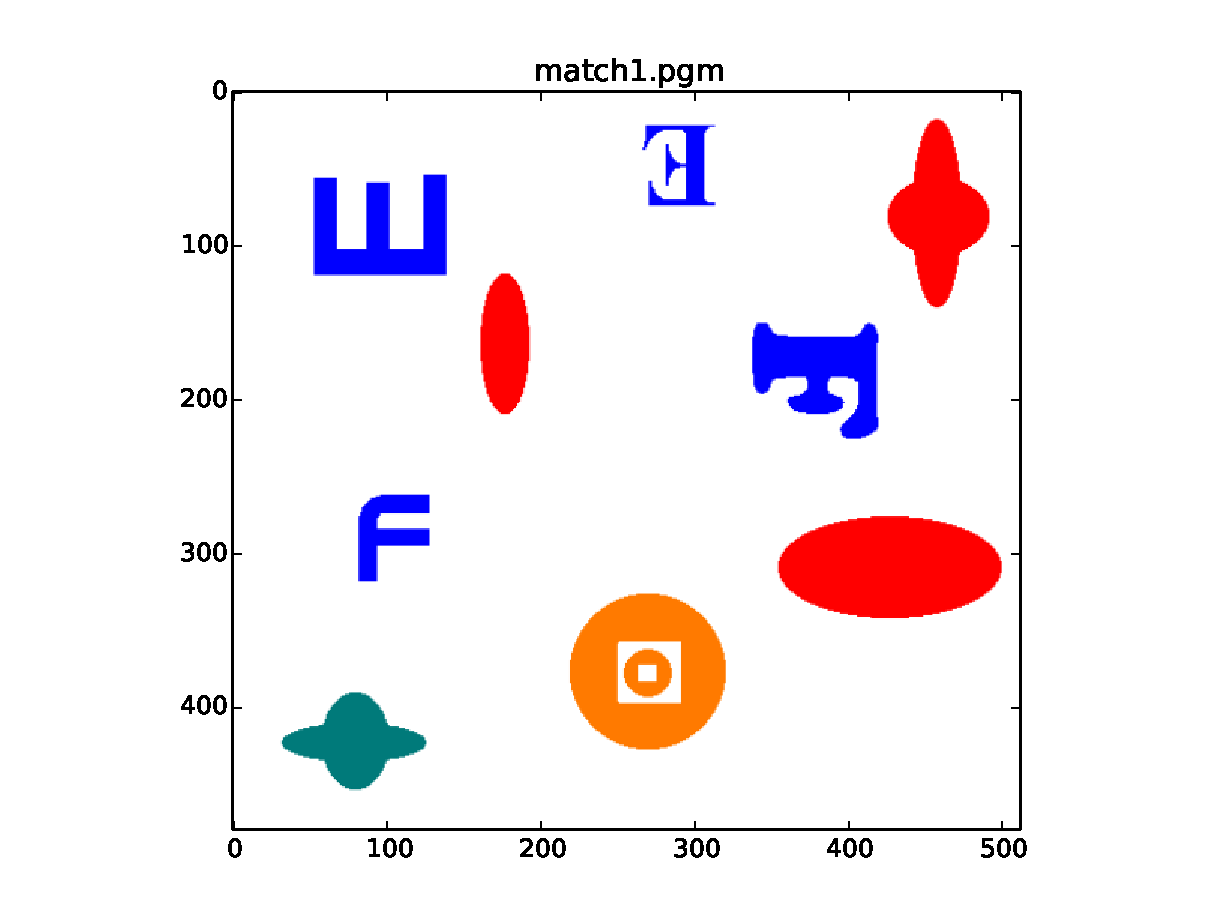
\includegraphics[width=.45\textwidth]{./figure/match1_pgm-0} 
\label{fig:class:02:match1} } 
\subfigure[Testing 2]{
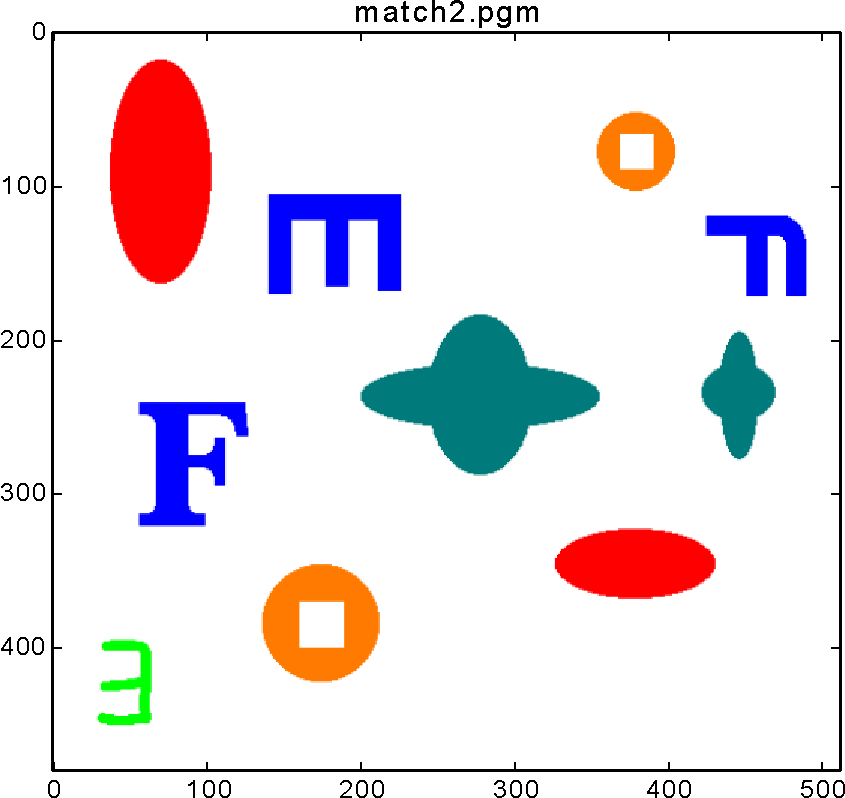
\includegraphics[width=.45\textwidth]{./figure/match2_pgm-0} 
\label{fig:class:02:match2} }
\caption{Classifications on \emph{train1.pgm}, \emph{train2.pgm}, \emph{match1.pgm} and \emph{match2.pgm}.}
\label{fig:class:02}
\end{figure}





\bibliography{reference}
\bibliographystyle{plain}

\end{document}